% *******************************************************************************
% * Copyright (c) 2008 by Elexis
% * All rights reserved. This document and the accompanying materials
% * are made available under the terms of the Eclipse Public License v1.0
% * which accompanies this distribution, and is available at
% * http://www.eclipse.org/legal/epl-v10.html
% *
% * Contributors:
% *    G. Weirich
% *
% *  $Id: elexis-privatrechnung.tex 3667 2008-02-08 15:09:40Z rgw_ch $
% *******************************************************************************

\documentclass[a4paper]{scrartcl}
\usepackage{german}
\usepackage[utf8]{inputenc}
\usepackage{makeidx}
\makeindex
% Hier ein etwas skurriler Block, der dazu dient, die Unterschiede
% zwischen pdflatex und latex auszubügeln
% Grafiken müssen als png oder gif (für pdflatex) und als eps (für Latex)
% vorhanden sein. Die Endung kann man beim \includegraphics jeweils weglassen,
% das System nimmt je nach Renderer die geeignete Variante.

\newif\ifpdf
\ifx\pdfoutput\undefined
	\pdffalse              	%normales LaTeX wird ausgeführt
\else
	\pdfoutput=1
	\pdftrue               	%pdfLaTeX wird ausgeführt
\fi

\ifpdf
	\usepackage[pdftex]{graphicx}
	\DeclareGraphicsExtensions{.pdf,.jpg,.png}
\else
	\usepackage[dvips]{graphicx}
	\DeclareGraphicsExtensions{.eps}
\fi

\usepackage{floatflt}
\usepackage{wrapfig}
\usepackage[]{hyperref}
\usepackage{color}
\begin{document}
\title{Elexis-Privatrechnung}
\author{Gerry Weirich}
\maketitle

\section{Einführung}
Dieses Plugin ermöglicht die Entwicklung und Einbindung von eigenen bzw. nicht als eigene Plugins erhältlichen Diagnosesystemen. Das Plugin ist dabei bewusst offen gehalten, ermöglicht also nicht nur medizinische Diagnosen, sondern jede Art von Dienstleistsgründen zu erfassen.

\section{Vorbereitung}
\subsection{Definition der Leistungen}
Sie benötigen eine Tabelle, in der Sie Ihre Diagnosen festgehalten haben. Dies kann eine Excel-Tabelle oder eine .csv-Datei sein. Diese muss den folgenden Aufbau haben:
\medskip
\begin{tabular}[h]{|r|r|r|r|}
\hline Gruppe & Kürzel & Text & Erläuterung\\
\hline
\end{tabular}

\medskip
Beispiel s. Abb. \ref{fig:diag}
\begin{figure}
  % Requires \usepackage{graphicx}
  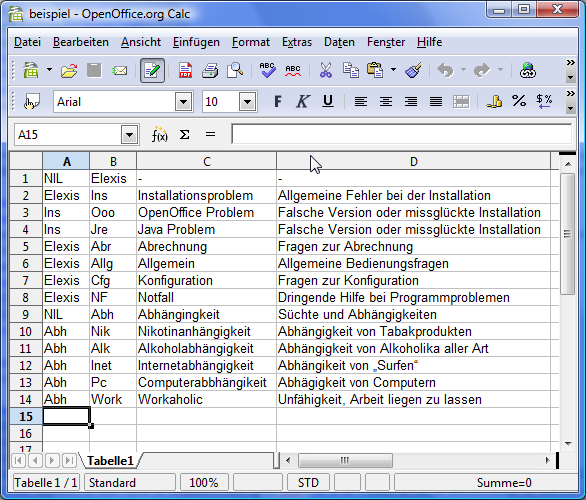
\includegraphics[width=0.9\textwidth]{diagnose_1}\\
  \caption{Beispiel-Diagnosesystem}\label{fig:diag}
\end{figure}


\medskip

Erläuterung: Der Inhalt der Tabelle wird als hierarchische bzw. baumartige Struktur (Vgl. Tessiner Code oder Tarmed) aufbereitet. Das heisst, jedes Element hat genau ein Eltern-Element und kann kein oder beliebig viele Unterelemente haben. Nur die Elemente der obersten Ebene haben kein Elternelement.

Die erste Spalte der Tabelle deklariert nun das Elternelement der betreffenden Leistung. NIL bedeutet, dass dieses Element zur obersten Ebene gehört. Ansonsten können die Bezeichnungen frei gewählt werden.

\subsection{Import}
Die so erstellte Tabelle kann nun nach Elexis importiert werden: Sofern das Eigendiagnose-Plugin installiert ist, erscheint in der 'Codes' View (in der Perspektive 'Codes') die entsprechende Seite 'Eigendiagnose' .

Wenn Sie im ViewMenu (Dreieck rechts oben) auf 'Import' Klicken, können Sie die csv- oder xls-Tabelle mit Ihrem Codesystem einlesen. \footnote{Änderungen können Sie nachträglich auch direkt in der codes-View vornehmen.} Danach stehen Ihnen Ihre selbstdefinierten Diagnosen wie jedes andere Codesystem zur Verfügung.


\end{document} 